% Figure: CPG verdict detectability map. For a top-of-leaderboard oracle
% rate (0.94), the boundary is the smallest oracle-minus-learned success-rate
% gap whose Agresti-Caffo CI clears zero at a given per-arm n -- i.e. the gap
% the five-branch verdict can actually commit on. Below the curve the gate
% returns INCONCLUSIVE; above it the ranking is decidable.
%
% Boundary computed by wmel.metrics.detectable_gap_at_n(0.94, 0.94 - g, n);
% values baked here so the figure is self-checking:
%   n:   10    20    30    50    75   100   150   200   300   500   1000
%   g: 0.415 0.260 0.195 0.140 0.110 0.090 0.070 0.060 0.045 0.035 0.025
%
% Annotated points (both at n=100): a leaderboard near-tie (gap 0.02) sits in
% the INCONCLUSIVE region; a wider gap (0.16) is decidable. Matches the
% leaderboard-gap audit in results/power_analysis.json.
\begin{figure}[t]
  \centering
  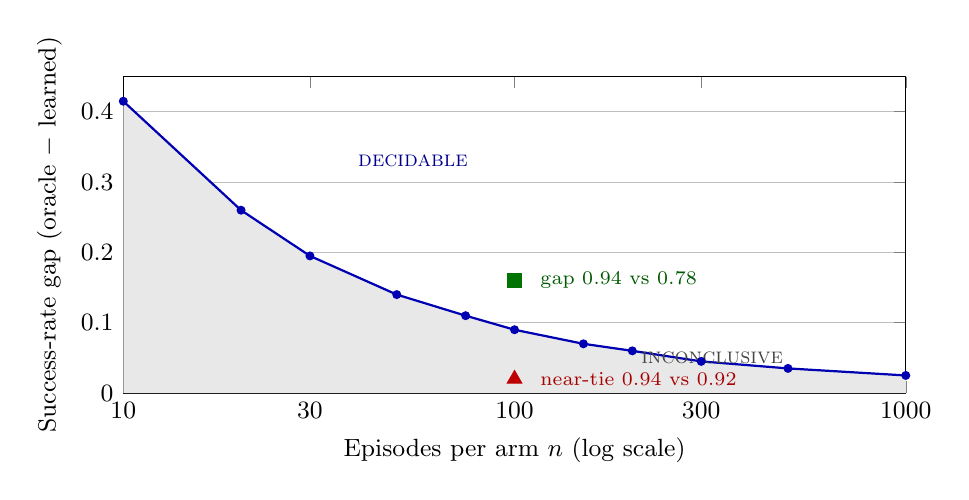
\begin{tikzpicture}
    \begin{axis}[
        width=0.95\columnwidth,
        height=5.6cm,
        font=\small,
        xmode=log, log basis x=10,
        xmin=10, xmax=1000,
        xtick={10, 30, 100, 300, 1000},
        xticklabels={$10$, $30$, $100$, $300$, $1000$},
        xlabel={Episodes per arm $n$ (log scale)},
        ymin=0, ymax=0.45,
        ytick={0, 0.1, 0.2, 0.3, 0.4},
        ylabel={Success-rate gap (oracle $-$ learned)},
        ymajorgrids=true,
        clip=false,
      ]
      % INCONCLUSIVE region: below the boundary (shade to the x-axis).
      \addplot[draw=none, fill=gray!18] coordinates {
        (10, 0.415) (20, 0.260) (30, 0.195) (50, 0.140) (75, 0.110)
        (100, 0.090) (150, 0.070) (200, 0.060) (300, 0.045) (500, 0.035) (1000, 0.025)
      } \closedcycle;
      % The decidability boundary itself.
      \addplot[color=blue!70!black, thick, mark=*, mark size=1.2pt] coordinates {
        (10, 0.415) (20, 0.260) (30, 0.195) (50, 0.140) (75, 0.110)
        (100, 0.090) (150, 0.070) (200, 0.060) (300, 0.045) (500, 0.035) (1000, 0.025)
      };
      % Region labels.
      \node[font=\footnotesize, gray!55!black] at (axis cs:320, 0.05) {\textsc{inconclusive}};
      \node[font=\footnotesize, blue!55!black] at (axis cs:55, 0.33) {\textsc{decidable}};
      % Annotated leaderboard points at n=100.
      \addplot[only marks, mark=triangle*, mark size=3pt, color=red!75!black]
        coordinates {(100, 0.02)};
      \node[font=\scriptsize, red!65!black, anchor=west] at (axis cs:110, 0.02)
        {near-tie $0.94$ vs $0.92$};
      \addplot[only marks, mark=square*, mark size=2.6pt, color=green!45!black]
        coordinates {(100, 0.16)};
      \node[font=\scriptsize, green!35!black, anchor=west] at (axis cs:110, 0.16)
        {gap $0.94$ vs $0.78$};
    \end{axis}
  \end{tikzpicture}
  \caption{Verdict detectability map at oracle rate $0.94$. The curve is the smallest oracle-minus-learned success-rate gap whose Agresti--Caffo $95\%$ CI clears zero at a given per-arm $n$ (computed by \texttt{detectable\_gap\_at\_n}). Below it the gate returns \textsc{inconclusive}; above it the ranking is decidable. A leaderboard near-tie ($0.94$ vs $0.92$, gap $0.02$) reported at $n = 100$ (red triangle) sits inside the \textsc{inconclusive} region -- the ordering is not supported by its own sample size; a wider gap ($0.94$ vs $0.78$, green square) is decidable at the same $n$. A point estimate cannot show which side of this boundary a reported ranking sits on.}
  \label{fig:power_detectability}
\end{figure}
